\documentclass[a4paper,12pt]{article}
\usepackage[utf8]{inputenc}
\usepackage[spanish]{babel}
\usepackage{color}
\usepackage{parskip}
\usepackage{graphicx}
\usepackage{multirow}
\usepackage{listings}
\usepackage{vmargin}
\usepackage{subfigure}
\graphicspath{ {imagenes/} }
\definecolor{mygreen}{rgb}{0,0.6,0}
\definecolor{lbcolor}{rgb}{0.9,0.9,0.9}
\usepackage{epstopdf}
     
\lstset{
backgroundcolor=\color{lbcolor},
    tabsize=4,    
%   rulecolor=,
    language=[GNU]C++,
        basicstyle=\tiny,
        aboveskip={1.5\baselineskip},
        columns=fixed,
        showstringspaces=false,
        extendedchars=false,
        breaklines=true,
        prebreak = \raisebox{0ex}[0ex][0ex]{\ensuremath{\hookleftarrow}},
        frame=single,
        showtabs=false,
        showspaces=false,
        showstringspaces=false,
        identifierstyle=\ttfamily,
        keywordstyle=\color[rgb]{0,0,1},
        commentstyle=\color[rgb]{0.026,0.112,0.095},
        stringstyle=\color{red},
        numberstyle=\color[rgb]{0.205, 0.142, 0.73},
%        \lstdefinestyle{C++}{language=C++,style=numbers}’.
}

\begin{document}



\begin{titlepage}

\begin{center}
\vspace*{-1in}

\begin{large}
UNIVERSIDAD NACIONAL DE SAN AGUSTÍN\\
\vspace*{0.15in}
ESCUELA PROFESIONAL DE CIENCIA DE LA COMPUTACIÓN\\
\vspace*{0.15in}
\end{large}
\begin{figure}[htb]
\centering

\includegraphics[scale=0.13]{logo.pdf}
\end{figure}
\vspace*{0.15in}
\begin{large}
TEMA:\\
\end{large}
\vspace*{0.2in}
\begin{Large}
\textbf{ANÁLISIS Y RESULTADOS} \\
\end{Large}
\vspace{8mm}

\begin{large}
Curso:\\
\end{large}
\vspace*{0.2in}
\begin{Large}
\textbf{ALGORITMOS PARALELOS} \\
\end{Large}

\vspace{8mm}

\begin{large}
\textbf{Presentado por:}\\

\begin{flushleft}

\hspace{7cm} Christofer Chávez Carazas \\

\end{flushleft}
\end{large}
\vspace{4cm}
\rule{80mm}{0.1mm}\\
\vspace*{0.1in}

\begin{large}
Arequipa - Perú \\
2017 \\
\end{large}
\end{center}
\end{titlepage}

  

\section{Descripción del Problema}

Comparar y analizar dos algoritmos para multiplicar matrices (Simple Matrix Multiplication / Tiled Matrix Multiplication)
en función del tiempo, los caché misses y la distancia de acceso a la memoria.

\section{Especificaciones del Experimento}

Ambos algoritmos están escritos en el lenguaje C. Para el experimento se generan dos matrices de $n$ x $n$ con números
aleatorios comprendidos entre 0 y 100. Dentro del tiempo calculado sólo se toma en cuenta la multiplicación
de las matrices (Los bucles anidados), no se toma en cuenta la creación de las matrices ni ninguna otra operación fuera
de la multiplicación de las matrices.
Para cada tamaño cada algoritmo se ejecutó cinco veces y se sacó el promedio de los tiempos. \\
Se utilizó valgrind y kcachegrind para ver el manejo de la memoria de ambos algoritmos, para esto se utilizaron matrices
de 700x700.

\section{Resultados y Análisis}

En la Figura \ref{res_fig} se muestra un gráfico con el tiempo de demora de los algoritmos respecto
al tamaño de las matrices. Claramente se observa que el algoritmo Tiled es más rápido que el algoritmo Simple cuando
el tamaño aumenta. Esto se debe a la gran diferencia que hay entre los caché misses que cada algoritmo produce; en
la Figura \ref{cache1} (Algoritmo Simple) y en la Figura \ref{cache2} (Algoritmo Tiled) esta remarcado el número de
caché misses. \\
El Algoritmo Tiled divide la matriz en bloques más pequeños, de tal manera que una fila de esos bloques quepa
en una línea de caché y poder utilizar esa fila lo más que se pueda, de modo que los caché misses se reducan considerablemente.
En este experimento se supuso un tamaño de línea de caché de 64 bytes. Ya que los enteros ocupan 4 bytes, las divisiones
hechas en el experimento son de 16 números por bloque. \\
El Algoritmo Simple no divide la matriz. Si el tamaño de una fila es más grande que el tamaño de una línea de caché,
al querer utilizar esa fila para la multiplicación, se generan muchos más caché misses.

\begin{figure}
 \centering
 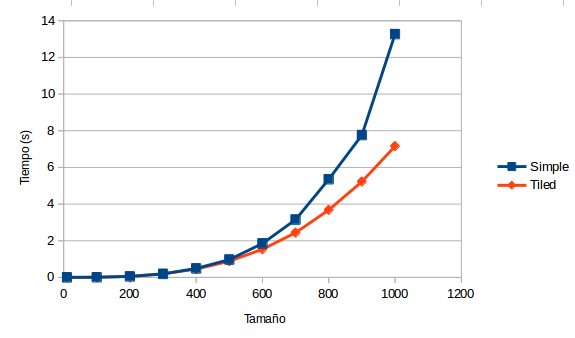
\includegraphics[scale=0.6]{Grafico_res.png}
 \caption{Resultados de las ejecuciones}
 \label{res_fig}
\end{figure}

\begin{figure}
  \centering
  \subfigure[Caché misses del algoritmo Simple]
    {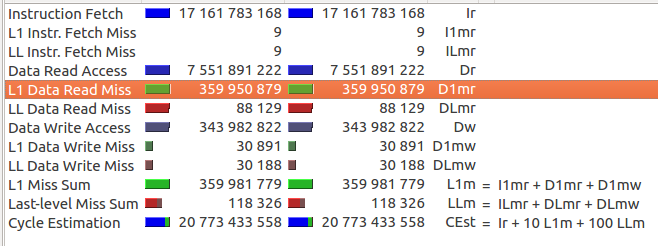
\includegraphics[scale=0.5]{cache1.png}
    \label{cache1}
   }
  \subfigure[Caché misses del algoritmo Tiled]{
    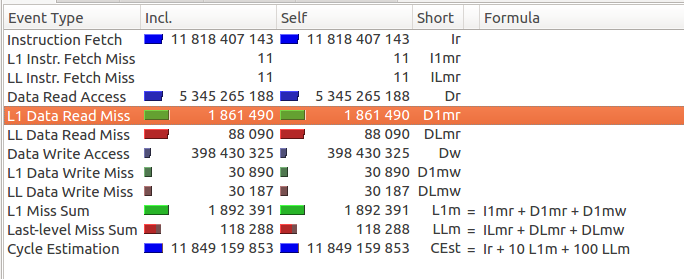
\includegraphics[scale=0.5]{cache2.png}
    \label{cache2}
   }
  \caption{Resultados del Kcachegrind}
\end{figure}

\newpage

\section{Conclusiónes}

\begin{itemize}
 \item Es importante tener nocion de cómo se maneja la memoria para poder optimizar los algortimos o programas.
 \item Los caché misses influyen mucho en el tiempo de ejecución de un algoritmo o programa.
 \item En el problema de la multiplicación de matrices óptima, el algoritmo Tiled es una buena forma de aumentar
 la rapidez, aunque teóricamente sigue teniendo un costo computacional de $O(n^{3})$.
\end{itemize}

\begin{thebibliography}{adasda}
  \bibitem{A} \textsc{Peter S. Pacheco} \textit{An introduction to parallel programming}
  \bibitem{B} \textsc{Lam, Monica S.; Rothberg, Edward E.; Wolf, Michael E.} (1991) \textit{The Cache Performance and Optimizations of Blocked Algorithms.}
\end{thebibliography}


\end{document}
